\RequirePackage{luatex85}
\documentclass[border = 1 cm]{standalone}
\usepackage{tikz}
\usetikzlibrary{shapes}
\usepackage{xcolor}
%You can modify your color here%

\begin{document}
\rotatebox{0}{
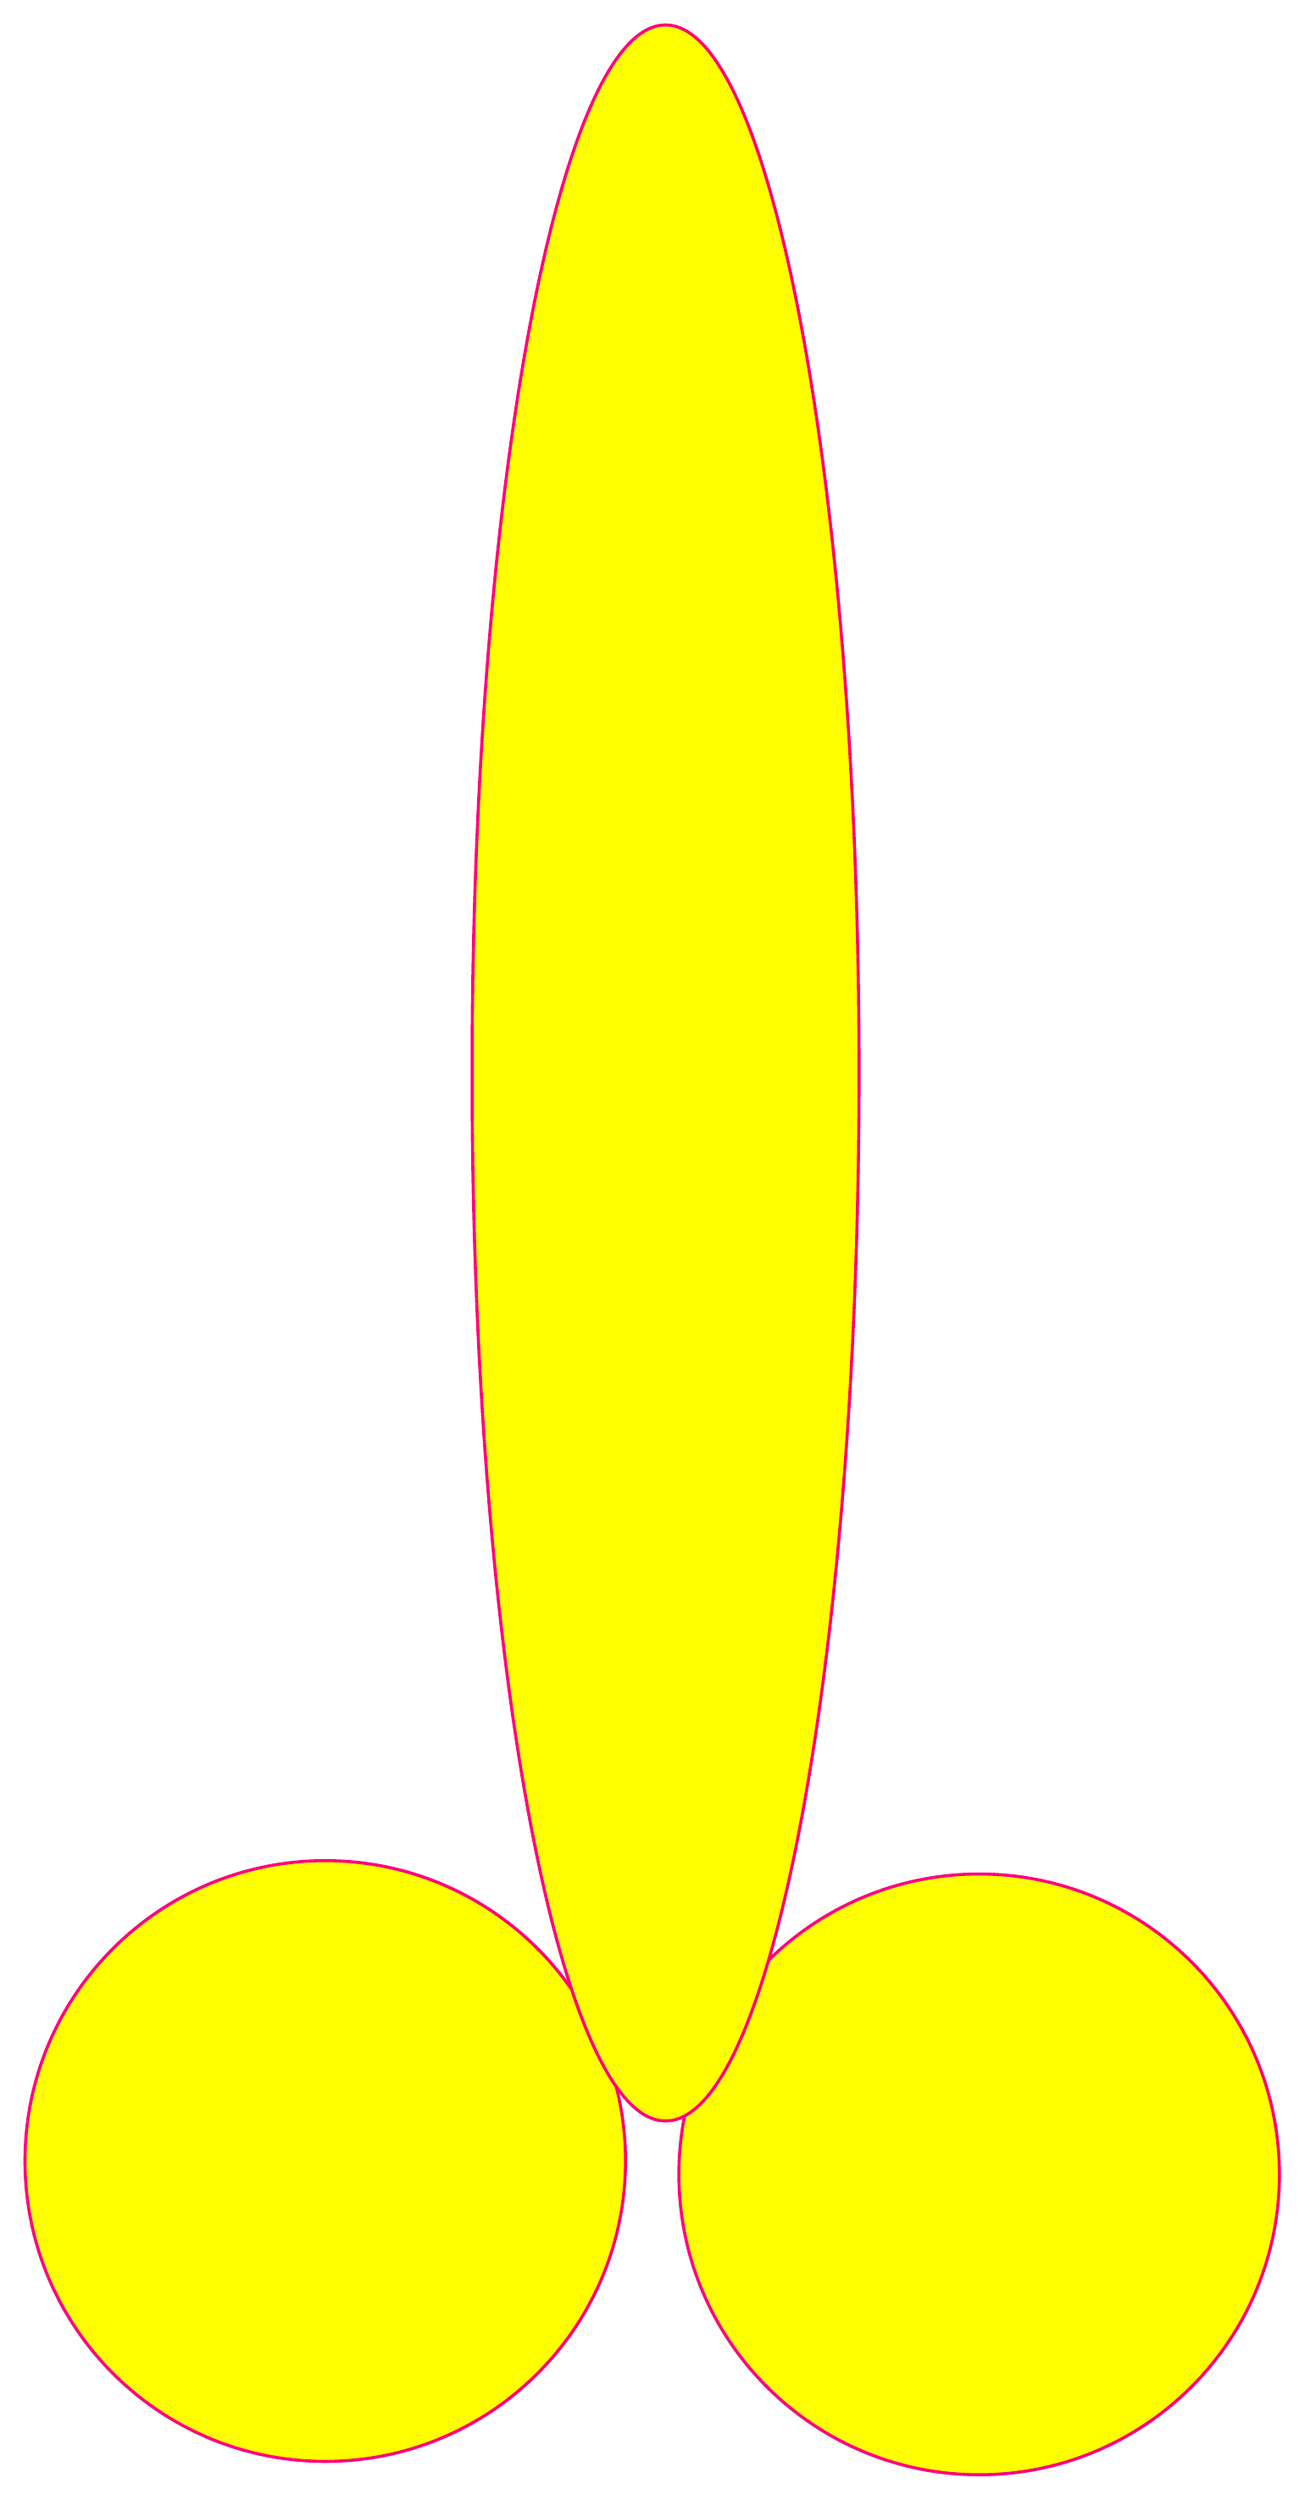
\begin{tikzpicture}[xscale=1,yscale=1]
\definecolor{linecolor}{RGB}{255,0,123} % Definition of the line color
\definecolor{fillcolor}{RGB}{255,255,0} % Definition of the fill color
\draw[draw=linecolor,fill=fillcolor,line width=1.3pt] (26.0,14.0) circle (4.5); % Draw a circle of radius 4.5 at the coordonates (26.0;14.0)
\definecolor{linecolor}{RGB}{255,0,123} % Definition of the line color
\definecolor{fillcolor}{RGB}{255,255,0} % Definition of the fill color
\draw[draw=linecolor,fill=fillcolor,line width=1.3pt] (35.8,13.8) circle (4.5); % Draw a circle of radius 4.5 at the coordonates (35.8;13.8)
\definecolor{linecolor}{RGB}{255,0,123} % Definition of the line color
\definecolor{fillcolor}{RGB}{255,255,0} % Definition of the fill color
\draw[draw=linecolor,fill=fillcolor,line width=1.3pt] (31.1,30.3) ellipse (2.9 and 15.7); % Draw an ellipse with a horizontal length of 2.9 and a vertical length of 15.7 at the coordonates (31.1;30.3)

\end{tikzpicture}
}
 
\end{document}